\documentclass[a4paper]{article}
\usepackage[utf8]{inputenc}
\usepackage[russian]{babel}
\usepackage{listings}
\usepackage[a4paper]{geometry}
\usepackage{indentfirst}
\usepackage{graphicx}
\usepackage{caption}
\usepackage{float}
\usepackage{amssymb}
\usepackage{physics}

\begin{document}

\title{Лабораторная работа 6 по курсу <<Нелинейная динамика и её приложения>>. \\Отчёт.}
\author{Владислав Соврасов\\ 381503м4}
\date{}
\maketitle

\section{Построение бифуркационной диаграммы логистичекого отображения}

Отображение \(x_{n+1}=(r-x_n)x_n\) называется логистическим. Известно, что при \(r\in [0;3)\)
оно имеет единственную устойчивую неподвижную точку, а при \(r\in [3;r_\infty),r_\infty<4\)
претерпевает бесконечно монго бифуркаций удвоения периода.

Для построения бифуркационной диаграммы необходимо найти неподвижние точки не только самого отображения,
но и его кратных композиций \(f\circ f, f\circ f \circ f, \dots\).
При нахождении неподвижных точек устойчвых циклов небольшой длины были с равномерным распределением сгенерированы
120 начальных точек из отрезка \([0;1]\), для каждой из которых вычислялись 1500 итераций логистического отображения.

\begin{figure}[H]
	\center
	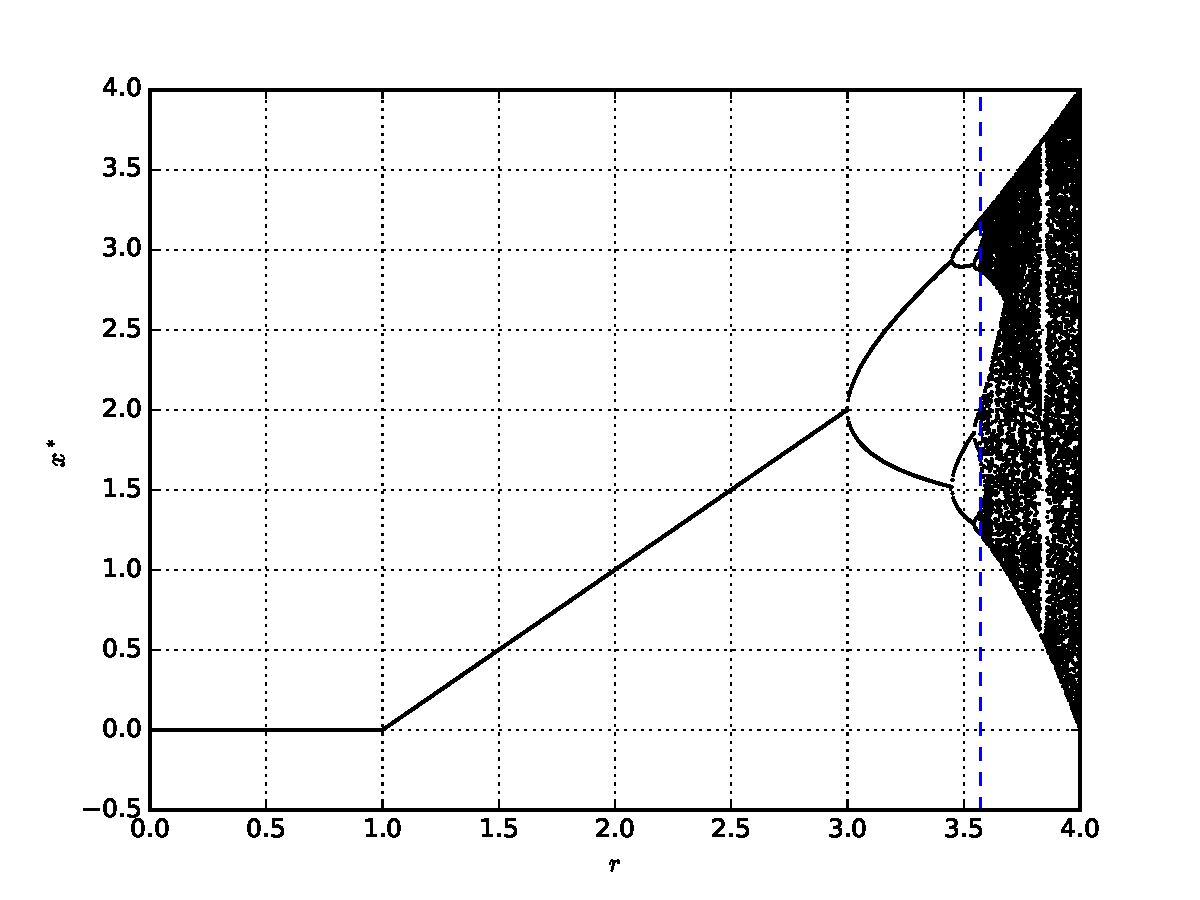
\includegraphics[width=0.75\textwidth]{../pictures/lab6_bifurcation_diagram.pdf}
	\caption{Бифуркационная диаграмма логистическго отображения}
	\label{fig:bifurcation_diagram}
\end{figure}

На рис. \ref{fig:bifurcation_diagram} представлена бифуркационная диаграмма при \(r\in[0;4]\).
На диаграмме чётко видны первые три бифуркации удвоения периода.
Вертикальной пунктирной линией обозначена оценка границы \(r_\infty\), после которой начинается
хаос (циклы конечного периода отсутствуют), но существует некоторых аттрактор.
При \(r>4\) аттрактор исчезает и продолжать диаграмму нет смысла.

\section{Исследование устойчивости логистичекого отображения на аттракторе}

Устойчивость какой-либо траектории отображения характеризуется Ляпуновским показателем
\begin{displaymath}
\lambda = \lim_{n \to \infty} \frac{1}{n}\sum_{k=1}^{n}\ln|f'(x_k)|
\end{displaymath}

Этот показатель зависит от начальной точки. Взяв достаточно много начальных точек,
можно рассматривать усреднённый показатель, который будет характеризовать устойчивость
траекторий аттрактора. Если параметр \(r\in [3;r_\infty)\), то средний показатель
должен быть неположительным, поскольку все траектории сходятся к неподвижной точке
какого-либо цикла, а значит устойчивы. На рис. \ref{fig:lyapunov_characteristic}
показан график зависимости средней по траекториям численной оценки \(\lambda\) от параметра \(r\).
Видно, что в моменты бифуркаций график подходит к \(0\), поскольку ассимптотическая
устойчивость неподвижных точек кратных отображений теряется. Также можно заметить, что
при \(r\), близких к \(4\), наблюдаются положительные значения оценки средней Ляпуновской величины,
что говорит о наличии хаоса.

В качестве грубой оценки положения точки \(r_\infty\) можно рассматривать первое, найденное
при построении графика значениe \(r\), для которого средняя оценка Ляпуновской величины положительна.
Указанным способом было получено, что \(r_\infty \approx 3.57\).

\begin{figure}[H]
	\center
	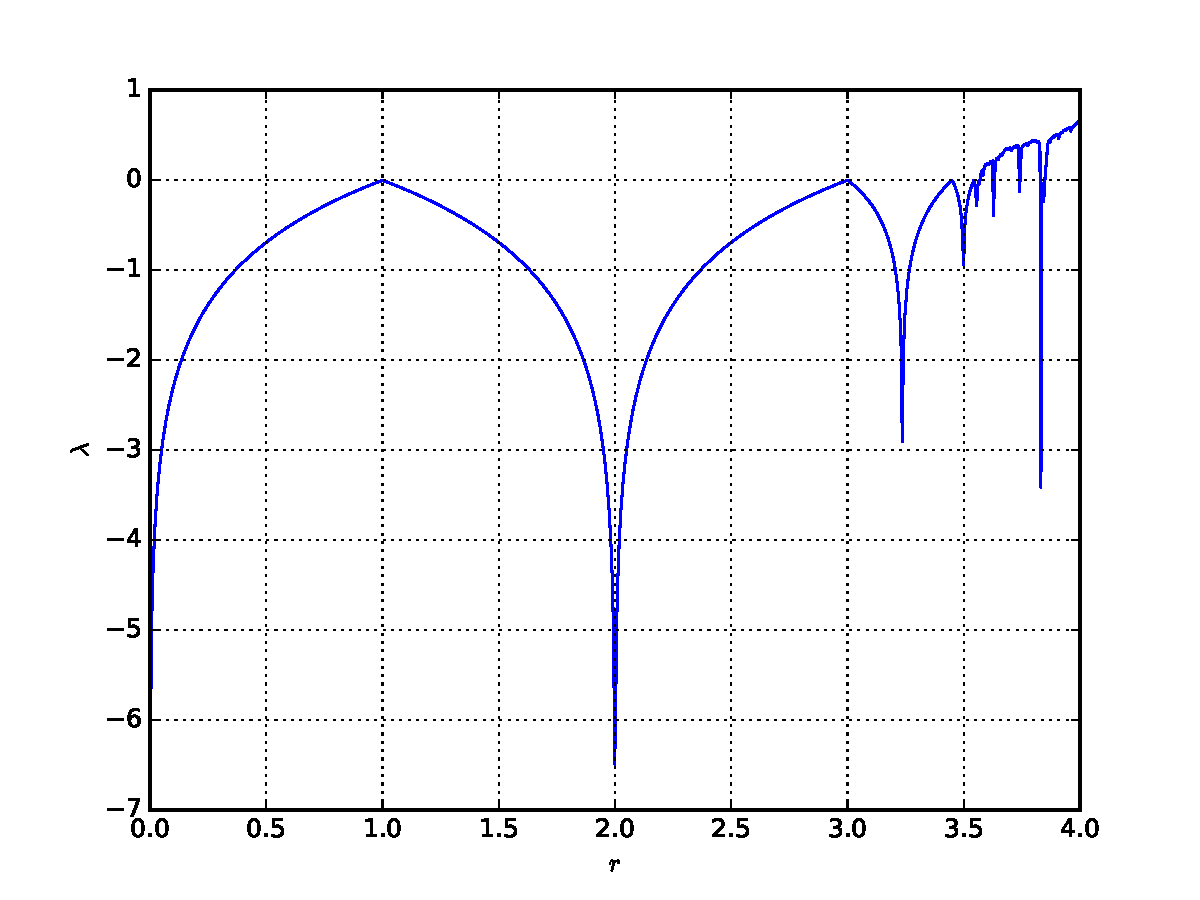
\includegraphics[width=0.75\textwidth]{../pictures/lab6_lyapunov_characteristic.pdf}
	\caption{Зависимость показателя Ляпунова от параметра отображения}
	\label{fig:lyapunov_characteristic}
\end{figure}

\section{Исходный код}
\lstinputlisting[language=Python, numbers=left]{../scripts/lab6.py}

\end{document}
